\documentclass{article}

\usepackage{arxiv}

\usepackage[utf8]{inputenc} % allow utf-8 input
\usepackage[T1]{fontenc}    % use 8-bit T1 fonts
\usepackage{hyperref}       % hyperlinks
\hypersetup{hidelinks = true}
\usepackage{url}            % simple URL typesetting
\usepackage{booktabs}       % professional-quality tables
\usepackage{amsfonts}       % blackboard math symbols
\usepackage{amsmath}
\usepackage{amssymb}
\usepackage{nicefrac}       % compact symbols for 1/2, etc.
\usepackage{microtype}      % microtypography
\usepackage{minted}

\usepackage[]{algorithm2e}

\usepackage{fancyvrb}
\usepackage{mathtools}
\DeclarePairedDelimiter{\ceil}{\lceil}{\rceil}

\usepackage{graphicx}
\usepackage{subcaption}

% ENVIRONMENTS
\usepackage{amsthm}
\theoremstyle{plain}
\newtheorem{definition}{Definition}[section]
\newtheorem{lemma}[definition]{Lemma}
\newtheorem{proposition}[definition]{Proposition}
\newtheorem{corollary}[definition]{Corollary}
\newtheorem{example}[definition]{Example}
\theoremstyle{remark}
\newtheorem{remark}[definition]{Remark}

% TEXT-MODE MACROS
\newcommand{\IE}{\mathbb{E}}
\newcommand{\IN}{\mathbb{N}}
\newcommand{\IR}{\mathbb{R}}
\newcommand{\IZ}{\mathbb{Z}}
\newcommand{\union}{\cup}
\newcommand{\Union}{\bigcup}
\newcommand{\code}{\texttt} % for use as \code{test()}
\newcommand{\defn}{\emph} % for use as \defn{...}

% MATH-MODE MACROS
\newcommand{\qtext}[1]{\quad\text{#1}\quad} % for use as \def{...} inside text
\newcommand{\ra}{\rightarrow}
\newcommand{\lra}{\longrightarrow}
\newcommand{\floor}[1]{\lfloor#1\rfloor}
\newcommand{\abs}[1]{|#1|}
\newcommand{\eps}{\epsilon}
\newcommand{\float}{\mathrm{float}}
\newcommand{\interval}[1]{[#1)}


\title{circllhist}

\subtitle{The Log-Linear Histograms for IT Infrastructure Monitoring}

\author{
  Heinrich Hartmann \\
  \texttt{heinrich.hartmann@circonus.com} \\
  Circonus \\
  \And
  Theo Schlossnagle \\
  \texttt{theo.schlossnagle@circonus.com} \\
  Circonus
}

\begin{document}

\maketitle

\begin{abstract}
  The circllhist histogram is a simple, fast and memory efficient data structure for capturing
  and processing large number of samples, that is particularly suited for applications in
  IT infrastructure monitoring.

  The circllhist allows arbitrary merging of pre-aggregated data without additional loss of accuracy,
  and the approximation of percentiles with low expected error and a-priori bounded maximal error.

  Open-source implementations are available for C/lua/python/Go/Java/JavaScript.
\end{abstract}

\tableofcontents

\input{part1.tex}

\clearpage
\section{Theory}

\begin{figure}
  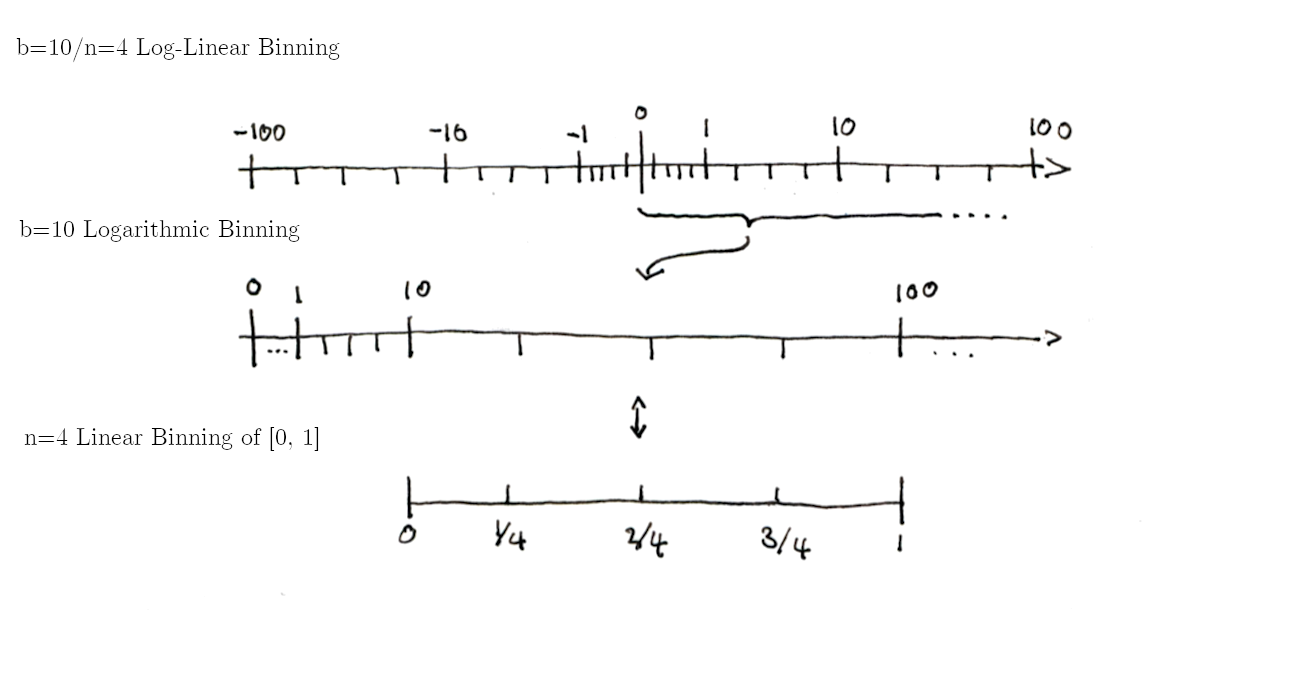
\includegraphics[width=\textwidth]{assets/LLBins.png}
  \caption{Construction of the Log-Linear Binning}
  \label{fig:llbins}
\end{figure}

The idea behind the circllhist is illustrated in Figure \ref{fig:llbins}, and quick to explain.
We start with a logarithmic binning of the real axes, that has bins at the powers of ten.
\begin{center}
  \begin{BVerbatim}
    ... 0.01, 0.1, 1, 10, 100, ...
  \end{BVerbatim}
\end{center}
We divide each logarithmic bin into $n=90$ equally spaced segments. In this way the bin boundaries
are preciesly the base-10, precision-2 floating point numbers:
\begin{center}
\begin{BVerbatim}
... 1.0,  1.1,  1.2,  ...   9.9,
     10,   11,   12,  ...    99,
    100,  110,  120,  ...   990, ...
\end{BVerbatim}
\end{center}
Those are the bin boundaries for the circllhist data structure.
When samples are inserted into the circllhist, we retain counts of the number of samples in each bin.
This information allows us to approximate the original location of the inserted samples with a
maximal relative error less than $5\%$.

In this section we develop an abstract theory of histograms to a degree that allows us to
formally define circllhist as a linear refinement of a logarithmic histogram structure,
and derive basic properties and error bounds.

\subsection{Binnings}

\begin{definition}
  Let $D \subset \IR$ be a connected subset of the real axes (e.g. $D=\IR, D=[0,1)$).
  A binning of $D$ is a collection of intervals $Bin[i], i \in I$, that are disjoint and collectively cover the binning domain $D$:
  \begin{align*}
    D = \Union_{i\in I} Bin[i] \qtext{and} Bin[i] \cap Bin[j] = \emptyset \qtext{for} i \neq j.
  \end{align*}
  The map that associates to each $x \in D$ the unique index $i$ so that $x \in Bin[i]$ is called
  binning map and is denoted as $bin(x) = i$.
\end{definition}

\begin{remark}
  The binning map $bin: D \ra I$ determines the binning via $Bin[i] = \{ x \in D \,|\, bin(x) = i \}$.
\end{remark}

\begin{example}
  The linear binning of $\IR$ is given by $I = \IZ$, with
  \begin{align*}
    Bin[i] = [i, i+1)  \qtext{and} bin(x)=\floor{x}
  \end{align*}
\end{example}

\begin{example}
  The length $n$ linear binning of $[0,1)$ is given by $I = \{0, \dots, n-1\}$, with
    \begin{align*}
      Bin^{Lin}_n[i]   = [ \frac{i}{n}, \frac{i+1}{n} )
      \qtext{and}
      bin^{Lin}_n(x) = \floor{x \cdot n}
    \end{align*}
\end{example}

\begin{example}
  The logarithmic binning with basis $b > 0$ of $\IR_{>0}$ is given by $I=\IZ$, with
  \begin{align*}
    Bin^{Log}_b[i] = [b^i, b^{i+1})
    \qtext{and}
    bin^{Log}_b(x)=\floor{\log_b(x)}
  \end{align*}
\end{example}

\begin{definition}\label{ref}
  Given a map $\alpha: I \ra J$, and a binning $(I, Bin)$, we can define a new binning
  $(J, Bin^*)$ by setting:
  \begin{align*}
    Bin^*[j] = \Union_{i, \alpha(i) = j} Bin[i], \qtext{and} bin^*(x) = \alpha(bin(x))
  \end{align*}
  In this situation we call $(J, Bin^*)$ a coarsening of $(I, Bin)$, and $(I, Bin)$ a refinement of $(J, Bin^*)$.
\end{definition}

\begin{definition}
  Given a binning $Bin[i], i\in I$ with half-open bins $Bin[i] = [a_i, b_i)$.
  The length-n linear refinement of $(I, Bin)$, is given by the index set $I \times \{0,\dots, n-1\}$,
  bins
  \begin{align}\label{eq:lref}
    L_nBin[i,j] = [ a_i + \frac{j}{n}(b_i - a_i), a_i + \frac{j+1}{n}(b_i - a_i) )
  \end{align}
\end{definition}

\begin{lemma}
  The binning map of the length-n linear refinement is given by:
  \begin{align}\label{eq:lrefmap}
    L_nbin(x) = ( bin(x), \floor{\frac{x - a_{bin(x)}}{b_{bin(x)} - a_{bin(x)}} \cdot n } ).
  \end{align}
\end{lemma}

\begin{proof}
  We have to show that $x \in L_nBin[ L_nbin(x) ]$ for all $x \in D$.
  Let $(i,j) = L_nbin(x)$.
  Since $i = bin(x)$, we know that $x \in [a_i, b_i)$.
  Now we consider the linear map $\phi(x) = (x-a_i)/(b_i-a_i)$ which maps $Bin[i]$ bijectively to $[0,1)$.
  We have $j = \floor{ n \phi(x) }$ by definition of $L_nbin(x)$.
  To show that $x \in L_nBin[ L_nbin(x) ]$ it suffices to verify
  that $\phi(x) \in \phi(L_nBin[i,j]) = [ \frac{j}{n}, \frac{j+1}{n} )$.
  And indeed,
  \begin{align*}
    \frac{j}{n} = \frac{\floor{ n \phi(x) }}{n} \leq \phi(x) <
    \frac{\floor{ n \phi(x) } + 1 }{n} =  \frac{j+1}{n}.
  \end{align*}
\end{proof}

\begin{lemma}
  The length-n linear refinement of a binning $(I, Bin)$ is a refinement in the sense of Definition \ref{ref}.
  The index map is given by $\alpha(i,j) = i$ for $i \in I$, $j \in \{0,\dots,n-1\}$.
\end{lemma}

\begin{proof}
  We have to show that $\Union_{j} L_nBin[i,j] = Bin[i]$, for all $i \in I$.
  Again we consider the linear bijection $\phi(x) = (x-a_i)/(b_i-a_i)$, which maps $Bin[i]$ to $[0,1)$ and $L_nBin[i,j]$ to $[j/n, (j+1)/n)$.
  Hence it suffices to show that $[j/n, (j+1)/n)$ cover $[0,1)$ for $j=0,\dots,n$ which is evident.
\end{proof}

Now we are in a position to define Log-Linear binnings.

\begin{definition}
  The base $b$, length $n$ log-liner binning of $\IR_{>0}$ is the length-n linear refinement of the base-b Logarithmic binning of $\IR_{>0}$.
\end{definition}

\begin{proposition}\label{prop:ll}
  Let $b,p$ be positive integers. The boundaries of the base $b$, length $n = b^p - b^{p-1}$ log-linear
  binning or $\IR_{>0}$ are precisely the base-p precision-p floating point numbers:
  \begin{align*}
    \float_{b,p}(e, d) = \frac{d}{b^{p-1}} \cdot b^e = d \cdot b^{e-p+1} \qtext{with} e \in \IZ, d \in \{ b^{p-1}, \dots, b^p - 1 \}
  \end{align*}
  The binning map is given by
  \begin{align*}
    LL_{n,b}bin(x) = (e(x), d(x) - b^{p-1}), \qtext{with} e(x) = \floor{\log_b(x)},\; d(x) = \floor{x \cdot b^{-e(x) + p - 1}}
  \end{align*}
  with values $e(x) \in \IZ$ and $d(x) \in \{b^{p-1}, \dots, b^{o} - 1\}$.
  This binning is also called base-b precision-p log-linear binning.
\end{proposition}

\begin{example}
  According to Proposition \ref{prop:ll}, the base-10 precision-1 binning has bin boundaries at
  \begin{align*}
      \{ d \cdot 10^e  \,|\, e \in \IZ, d \in \{ 1, \dots, 9 \} \} = \{ \dots 0.8, 0.9,\; 1, 2 \dots, 8, 9,\; 10, 20 \dots \}
  \end{align*}
  binning map
  \begin{align*}
    LL_{n,b}bin(x) = (e(x), d(x) - 1), \qtext{with} e(x) = \floor{\log_{10}(x)},\; d(x) = \floor{x / 10^{e(x)}}.
  \end{align*}
\end{example}

\begin{proof}
  To proof Proposition \ref{prop:ll}, we compute the log-linear bin boundaries using equation \ref{eq:lref}
  with $a_i = b^i, b_i = b^{i+1}$ and $n = b^p - b^{p-1}$:
  \begin{align*}
    LL_{b,n}Bin[e,j] &= [ b^e + \frac{j}{b^p - b^{p-1}}(b^{e+1} - b^e), b^e + \frac{j + 1}{b^p - b^{p-1}}(b^{e+1} - b^e) ) \\
      &= [ b^{e-p+1}(b^{p-1} + j), b^{e-p+1}(b^{p-1} + j + 1) ) \\
      &= [ d b^{e-p+1}, (d + 1) b^{e-p+1} )
  \end{align*}
  where we set $d = b^{p-1} + j$. If $j$ runs through $1 \dots n$, then $d$ runs through $b^{p-1},\dots, b^p -1$.
  This shows that the lower boundaries are exactly the base-b precision-p floating point numbers.
  For the upper boundary note, that the if $d=b^p-1$ then $(d+1)b^{e-p+1} = b^{p-1} b^{(e+1)-p+1}$ is again
  a base-b precision-p floating point number (with a larger exponent).

  The binning map can be explicitly calculated using Equation \ref{eq:lrefmap} as:
  \begin{align*}
    LL_{b,n}bin(x) &= (e(x), k(x)), \qtext{with} e(x) = \floor{\log_b(x)} \\
    k(x) & = \floor{ \frac{x - b^{e}}{b^{e+1} - b^e} (b^p - b^{p-1}) }
    = \floor{x \cdot b^{-e + p - 1}} - b^{p-1}
    = d(x) - b^{p-1}
  \end{align*}
  as claimed.
\end{proof}

\begin{definition}
  The circllhist binning is the base-10 precision-2 log-linear binning extended to the real axes,
  with bins:
  \begin{align*}
    CLLBin[+1,e,d] &= [ d \cdot {10}^{e-1}, (d + 1) 10^{e-1} ), \quad e \in \IZ, d \in \{ 10, \dots, 99 \} \\
    CLLBin[0,0,0]  &= \{ 0 \} \\
    CLLBin[-1,e,d] &= [ -d \cdot {10}^{e-1}, -(d + 1) \cdot 10^{e-1} ).
  \end{align*}
  The binning map is given by:
  \begin{align*}
    CLLbin(x)  &= (+1, e, d), e = \floor{\log_{10}(x)}, d = \floor{x \cdot 10^{-e - 1}} \\
    CLLbin(0)  &= (0, 0, 0) \\
    CLLbin(-x) &= (-1, e, d)
  \end{align*}
  for $x > 0$.
\end{definition}

\begin{proposition} \label{prop:rec}
  The binning map of the circllhist can be recursively computed as follows:

  \begin{figure}[h]
  \begin{cetner}
    \begin{BVerbatim}
  function CLLbin(x)
    if x == 0:
      return (0,0,0)
    if x < 0:
      (s, e, d) := CLLbin(-x)
      return (-1, e, d)
    if x < 10:
      return CLLbin(x * 10) - (0, 1, 0)
    if x > 100:
      return CLLbin(x / 10) + (0, 1, 0)
    else: # 10 <= x < 100:
      return (+1, 1, floor(x))
  end
    \end{BVerbatim}
  \end{cetner}
  \end{figure}

  In particular, the circllhist binning map can be computed without use of the logarithm function.
\end{proposition}

\begin{proof}
  The recursion terminates since every positive number $x$ can be brought into range $10 \leq x <
  100$ with a finite number of divisions or multiplications by $10$.  It's straight forward to
  verify that each case computes valid results assuming that the results of the recursive call are
  correct.
\end{proof}

\begin{remark}
  If $x,e$ are integers, than the binning map of the number $x \cdot 10^{e}$ can be computed without
  the use of floating point arithmetic as $CLLbin(x) + (0,e,0)$ using Algorithm \ref{prop:rec}.

  This is of practical relevance when used in an environment which do not have floating
  point arithmetic available. One example being nano-second latencies measured in the Linux kernel,
  or embedded devices.
\end{remark}

\subsection{Paretro Midpoints}

\begin{proposition} \label{prop:pdist}
  Given an interval $[a,b]$ in $\IR_{>0}$ the unique point $m$ in $[a,b]$ so that the maximal
  relative distance $rd(m, y) = |m-y|/y$ to all other points in $[a,b]$ is minimized
  by the paretro midpoint
  $m = 2ab / (a + b)$.

  The maximal relative distance to the paretro midpoint is is $(b - a) / (a + b)$
\end{proposition}

\begin{proof}
  We have to minimize the function $maxrd(x) = max_{y\in[a,b]} rd(x, y)$ over $[a,b]$.
  The maximum $max_{y\in[a,b]} rd(x, y)$ is attained either for $y = a$ or $y = b$,
  hence $maxrd(x) = max\{ rd(x,a), rd(x,b) \}$.

  Note that the function $f(x) = rd(x, a)$ is continues and strictly monotonically increasing on $[a,b]$, with $f(a) = 0, f(b) > 0$,
  and the function $g(x) = rd(x, b)$ is continues and strictly monotonically decreasing on $[a,b]$, with $g(a) > 0$ and $g(b) = 0$.
  The point $m$ is the unique point in $[a,b]$ where both functions are equal, with
  \begin{align*}
    rd(m, a) = \frac{b - a}{a + b} = rd(m, b)
  \end{align*}
  Now if $a \leq x < m$ then $rd(x, b) = g(x) > g(m)$ and so $maxrd(x) > maxrd(m) = g(m)$.
  Similarly if $m < x \leq b$ then $rd(x, a) = f(x) > f(m)$ and so $maxrd(x) > maxrd(m) = f(m)$.

  This shows that $x=m$ is the unique minimum of $maxrd(x)$ on $[a,b]$.
\end{proof}

The following proposition gives a probabilistic interpretation of the location of relative distance minimizing midpoint.
Recall, that the expected value of a uniformly distributed random variable $X \sim U[a,b]$ is the midpoint $\IE[X] = (a+b)/2$.

\begin{proposition}
  Given an interval $[a,b]$, and an a=2 paretro distributed random variable $X$, then
  \begin{align*}
    \IE[ X \, | \, X \in [a,b] \,] = 2ab / (a + b),
  \end{align*}
\end{proposition}

\begin{proof}
  The paretro distribution has density $p(x) =C \cdot 1/x^{a+1}$, for some positive constant $C$, so for $a=2$ we get
  \begin{align*}
    \IE[ X \, | \, X \in [a,b] \,] = \frac{\int_a^b x p(x) dx}{\int_a^b p(x) dx}
    = \frac{\int_a^b x^{-2}  dx}{\int_a^b x^{-3} dx} = 2 \frac{b^{-1} - a^{-1}}{b^{-2}- a^{-2}}
    = \frac{2}{b^{-1} + a^{-1}}
    = 2 \frac{ab}{a + b}
  \end{align*}
  which proves the claim.
\end{proof}

\begin{proposition}\label{prop:21}
  The maximal relative distance to a paretro midpoint in the circllhist binning is $1/21 \approx 4.76\%$.
\end{proposition}

\begin{proof}
  Substituting the bin boundaries into the formula given in Proposition \ref{prop:pdist} we find
  $(b - a)(a + b) = 1/(2d + 1)$ for the bin $CLLBin[e,d], e \in \IZ, d \in \{ 10, \dots, 99 \}$.
  This is minimized for $d = 10$ with a value of $1/21$ as claimed.
\end{proof}

\subsection{Histograms}

Once we have established our binnings. Histograms are easy to define.

\begin{definition}
  A histogram with domain $D \subset \IR$ is a binning $Bin[i],I$, together with a count function $H: I \ra \IN_{0}$.
\end{definition}

Given a dataset and a binning, we associate a histogram.

\begin{definition}
  Given binning $Bin[i],I$ of $D \subset \IR$, and a dataset $X = (x_1,\dots,x_n)$ with values in
  $D$, we define the histogram summary of $X$ as the histogram with binning $Bin[i],I$ and count
  function
  \begin{align*}
    H_X(i) = \# \{ j \, | \, x_j \in Bin[i] \, \}.
  \end{align*}
  This means, that $H_X(i)$ counts the number of points of $X$ lying in $Bin[i]$.
\end{definition}

Histograms can be freely merged without loosing information.

\begin{definition}
  Let $H_1, H_2$ be histograms for the same binning. The merged histogram $H_1 + H_2$ has count function:
  \begin{align*}
    (H_1+H_2)(i) = H_1(i) + H_2(i).
  \end{align*}
\end{definition}
The merge operation is clearly associative and commutative.

We can easily see that the histogram merge computes is compatible with merge (concatenation) of datasets:
\begin{proposition}
  Given binning $Bin[i],I$ of $D \subset \IR$, and two datasets $X = (x_1,\dots,x_n),Y=(y_1,...y_m)$ with
  values in $D$. Let $Z=(x_1, \dots, x_n, y_1, \dots, y_m)$ be the merged dataset, then $H_Z = H_X + H_Y$.
\end{proposition}

\begin{proof}
  We have
  \begin{align*}
    H_Z(i) &= \# \{ j \, | \, z_j \in Bin[i] \, \} =
    \# \{ j \leq n \, | \, x_j = z_j \in Bin[i] \, \} +
    \# \{ j > n \, | \, z_j = y_{j-n} \in Bin[i] \, \} \\
    &= H_X(i) + H_Y(i). \qedhere
  \end{align*}
\end{proof}

\subsubsection{Histogram Operations}

Given a histogram we can try to approximate statistics (means, percentiles, etc.) of the original dataset.
There are three strategies for doing so, that we have found valuable in practice:

\begin{enumerate}
\item Derive a probability distribution from a histogram (with uniform distribution inside the
  bins), and apply the statistics to this distribution.
\item Reconstruct the dataset by placing all points inside a bin at equally spaced distances.
\item Reconstruct the dataset by placing all points inside a bin into the paretro midpoints.
\end{enumerate}

From a theoretical perspective strategy (1) is the most natural, and gives generally good results
for data sampled from continues distribution (with density).
Strategy (3) is the simplest and gives a clear a-priori error bounds independent of the distribution of $X$.
Strategy (2) is mitigates between both approaches, and gives lower expected errors on a wide variety of
datasets and while avoiding large relative errors in case of single sample bins.

The current implementation of circllhist uses Strategy (3) to define sum, mean, stddev and moment estimation.
For percentile calculations Strategy (2) is used.

\begin{proposition}
  Let $X=(x_1,\dots,x_n), n>0$ be a dataset with values in $\IR_{>0}$, let $H$ be the circllhist summary of $X$.
  For each bin $Bin[i]$, let $c_i \in Bin[i]$ be the paretro midpoint. Let
  \begin{align*}
    count[H] = \sum_i H(i), \quad sum[H] = \sum_{i\in I} H(i) \cdot c_i, \qtext{and} mean[H] = sum[H] / count[H].
  \end{align*}
  then
  \begin{enumerate}
  \item $count[H] = count(X) = n$.
  \item The relative error $|sum[H] - sum(X)| / sum(X)$ is smaller than $1/21 \approx 4.76\%$.
  \item The relative error $|mean[H] - mean(X)| / mean(X)$ is smaller than $1/21 \approx 4.76\%$.
  \end{enumerate}
\end{proposition}

\begin{proof}
  The first claim follows immediately from the definition of $count[H]$, and $H(X)$.
  For the second claim, we have
  \begin{align*}
    sum[H] - sum(X) = \sum_{i\in I} H(i) \cdot c_i - \sum_j x_j
    = \sum_{i\in I} ( H(i) \cdot c_i - \sum_{j, x_j \in Bin[i]} x_j)
    = \sum_{i\in I} \sum_{j, x_j \in Bin[i]} (c_i - x_j)
  \end{align*}
  And hence,
  \begin{align*}
    |sum[H] - sum(X)| \leq \sum_{i,j, x_j \in Bin[i]} |c_i - x_j| \leq \sum_{j} \frac{1}{21} |x_j| = \frac{1}{21} \cdot sum(X),
  \end{align*}
  where we used \ref{prop:21} in second step.
  This shows the second claim.
  For the third claim follows from the second by extending the fraction with $1/n$.
\end{proof}

\subsubsection{Quantiles}

Quantiles can be approximated from histograms using any of the strategies outlined at the beginning
of the section.  Strategy (1) has the downside, that for $q$ close to $1$, the $q$-quantile will always
be near the high end of the largest bin with at least one sample in it. Often times this bin contains
only a single sample. In this case the worst case error of the full bin size can be easily assumed.

Strategy (3) has the downside, that expected errors for percentiles in the center of the distribution
are much larger than needed. For densely populated bins the uniform distribution is often a good
approximation, and can be used to estimate percentiles with high precision in typical cases.

Strategy (2) offers a welcome middle route. Instead of placing all samples at the (paretro) midpoint (3),
or smoothing them out with a uniform distribution (1), we place the samples at equally spaced position
within each bin. In this way, densely populated bins will be approximated by a near uniform distribution
and bins with only a single sample will be replaced by a single sample at the midpoint, reducing
the worst-case error to half the bin size.

\begin{definition}
  Given a histogram $H$ on a binning $Bin[i], i \in I$ we define the fair resampling $X$ of $H$ as follows.
  For each bin $Bin[i]$, with boundaries $a,b$ and count $H(i)=n$, we consider the points
  \begin{align*}
    x_{i,k} = a + \frac{k}{n+1} (b-a) \qtext{for} k=1,\dots,n
  \end{align*}
  and let $X = (x_{i,k} \,|\, i \in I, k = 1\dots,H(i))$. This is a dataset with $count[H]$ points.
\end{definition}

We now want to define the quantiles of a histogram as quantiles of the fair resampling of $H$.
Before we can do so we first need to clarify the quantile definition for datasets.
While there is only a single established quantile definition for probability distributions,
there are multiple different quantile definitions found in the wild.
A comprehensive list was compiled by Hyndman-Fan in 1996 \cite{HF1996}.
For our discussion the following two variants are relevant:

\begin{definition}
  Given a dataset $X=(x_1,\dots,x_n), n>0$ of real numbers, and a number $q \in [0,1]$.
  Let $x_{(1)} \leq x_{(2)} \leq \dots \leq x_{(n)}$ be the ordered version of $X$.
  We define the minimal type-I q-quantile as
  \begin{align*}
    Q^1_0(X) = x_{(1)} \qtext{and}  Q^I_q(X) = x_{(\ceil{q \cdot n})} \qtext{for} q > 0.
  \end{align*}
  We define the minimal type-VII quantile is given by:
  \begin{align*}
    Q^{7}_q(X) = x_{(\floor{q \cdot (n - 1)} + 1)}.
  \end{align*}
  The interpolated type-VII quantile is given by:
  \begin{align*}
    Q^{7i}_q(X) = \gamma \cdot x_{(\floor{q \cdot (n - 1)} + 1)} + (1-\gamma) \cdot x_{(\ceil{q \cdot (n - 1)} + 1)},
  \end{align*}
  where the interpolation factor $\gamma \in [0,1]$ is calculated as $q(n-1) - \floor{q(n-1)}$.
\end{definition}

This definition is consistent with the numbering in \cite{HF1996}.

* Type-1 quantiles are consistent with probability theory (empirical distribution function).

* Type-1 quantiles allow to derive precise statements about the lower counts, e.g.

> 95\% of all requests were served within 500ms IFF p95 < 500ms

This is not true for Type-7 quantiles, which make statments about 95% of (n-1) requests.

* Type-7 quantiles are most commonly found in software packages and used in dd-sketch, t-digest, hdr?!


\section{Implementation}


* Binning is fixed once and for all.
* Bins are represented as exponent (8bit) + mantissa (8bit?).
* Sparse encoding of histogram as list of bin+count pairs
* Fast insertion tricks

\section{Evaluation}

\clearpage
\subsection{Calibration}

\begin{figure}
   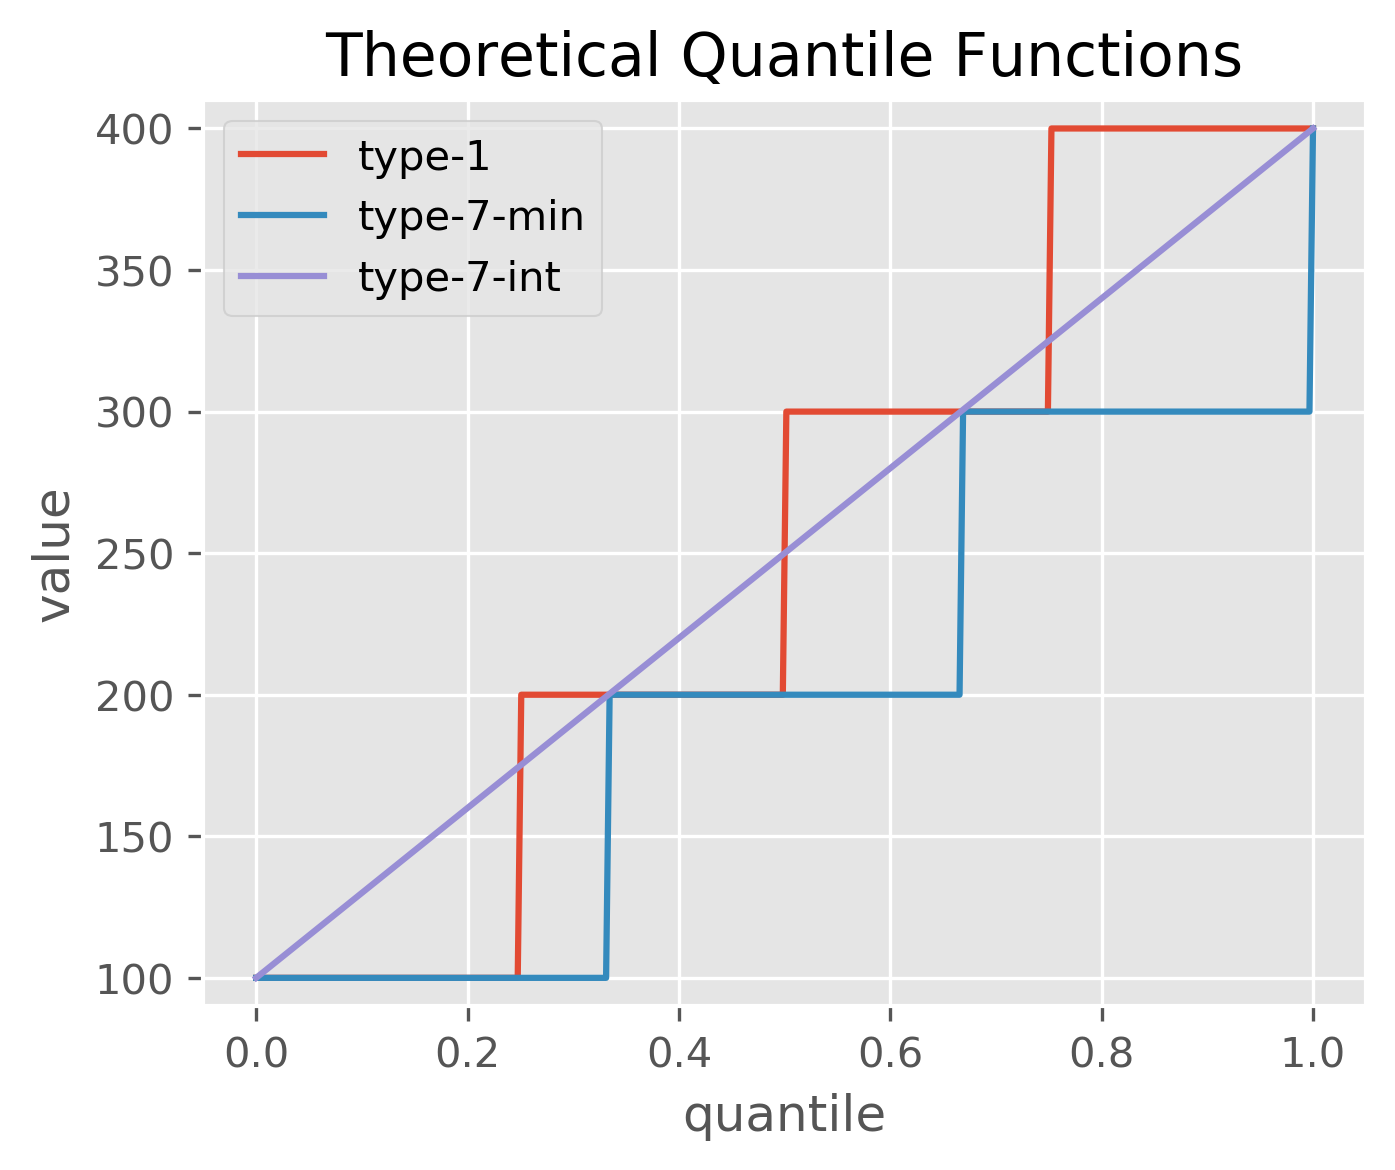
\includegraphics[width=\textwidth / 2]{evaluation/images/theoretical_quantile_comparison.png}
   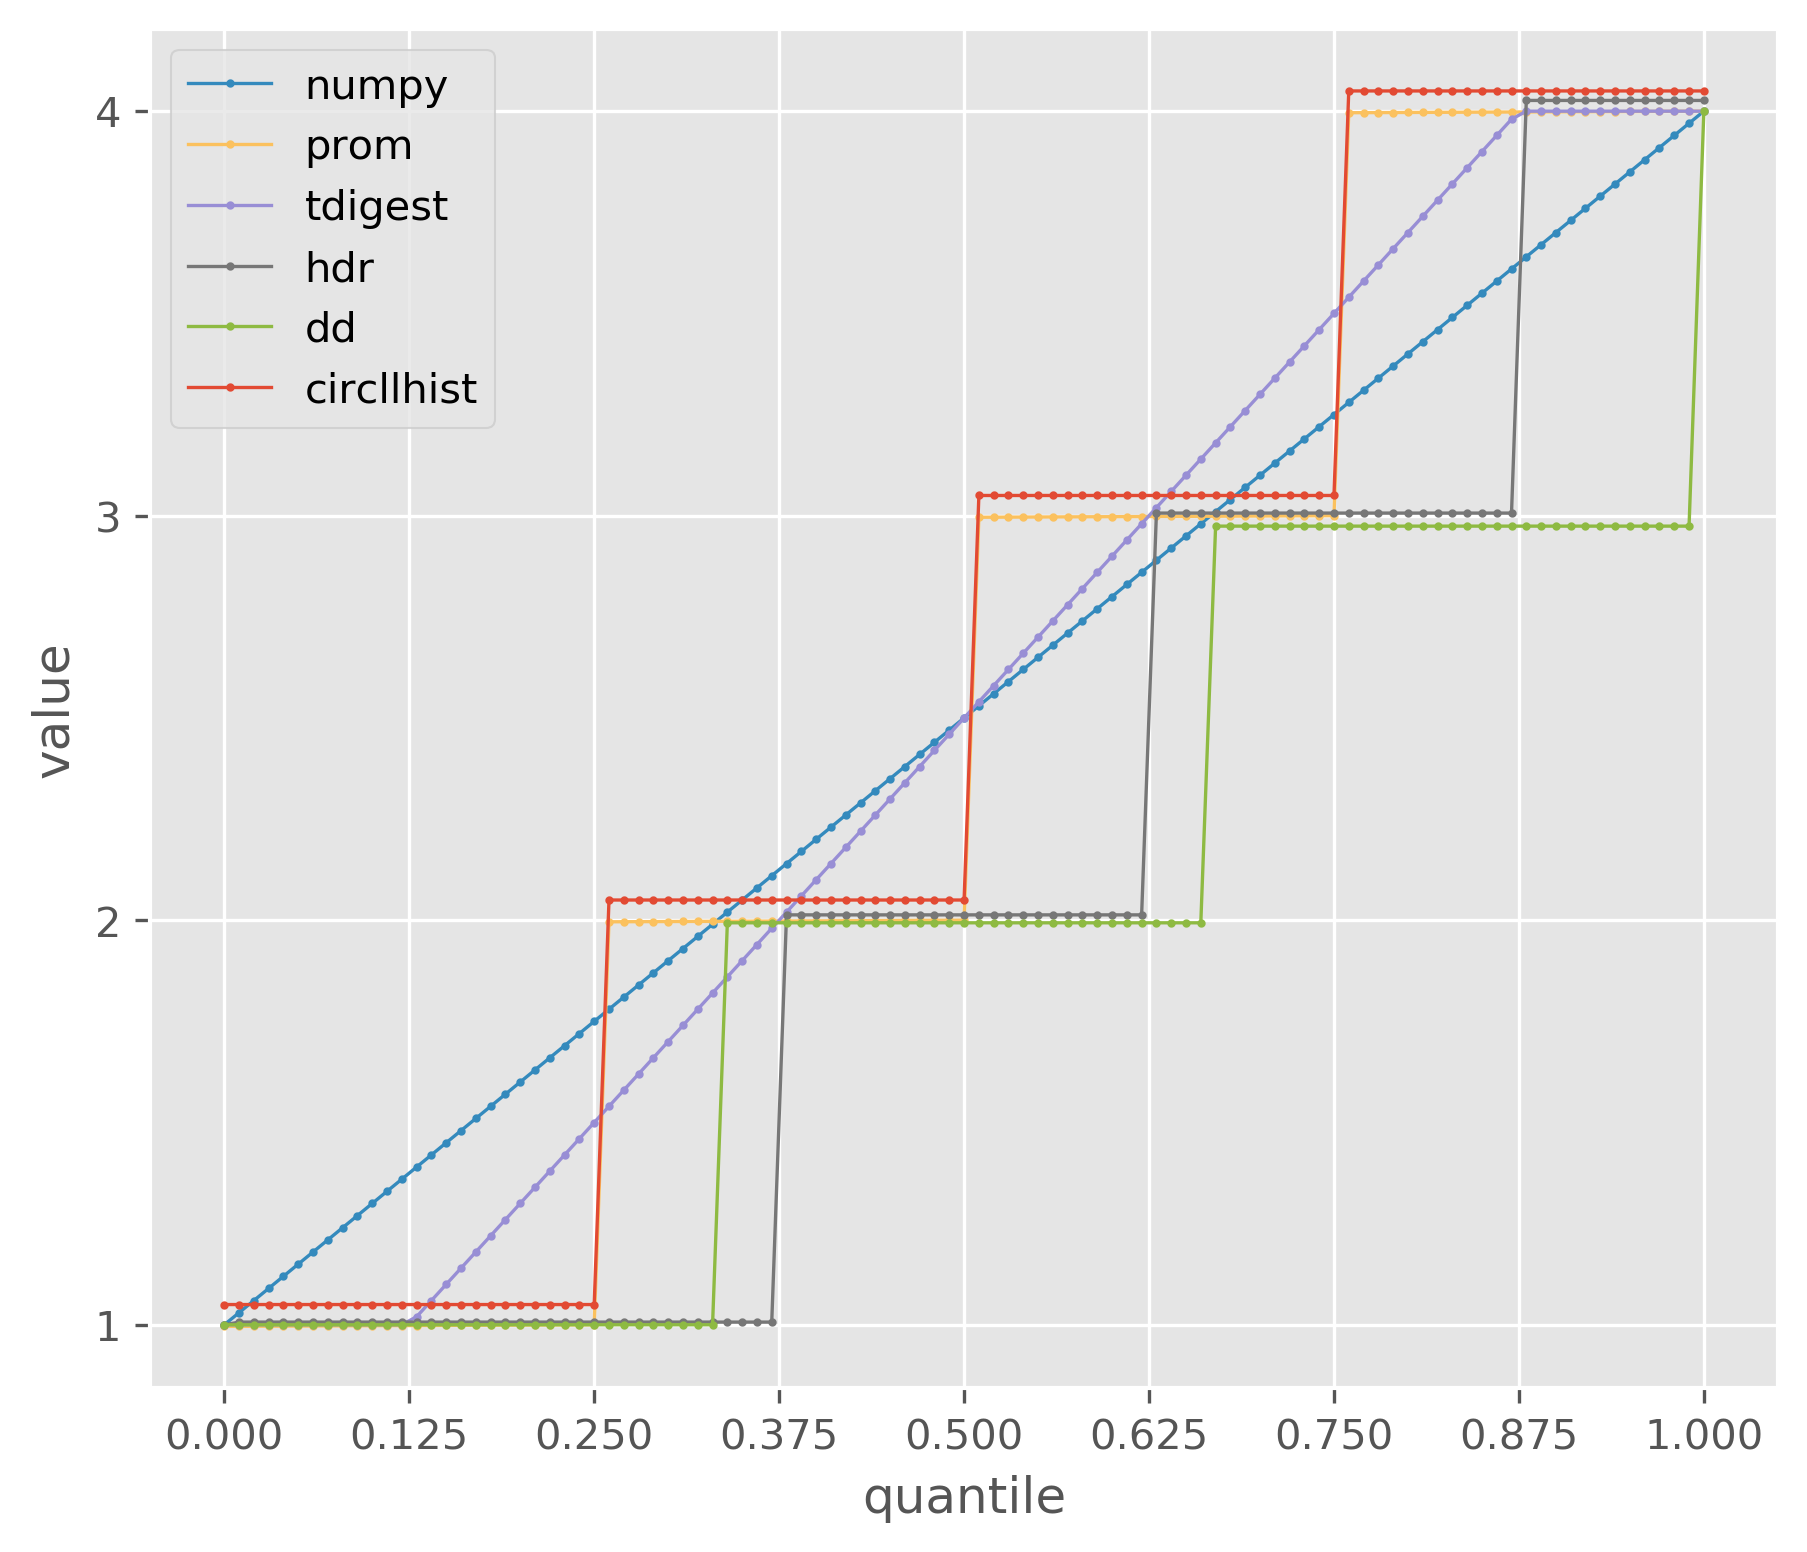
\includegraphics[width=\textwidth / 2]{evaluation/images/practical_quantile_comparison.png}
   \caption{Comparison of quantile functions for the data set $[100,200,300,400]$ }
\end{figure}

\begin{figure}
  \centering
  \begin{tabular}{lrrrrrrrrr}
\toprule
{} &  type-1 &  type-7-min &  type-7-int &    prom &     hdr &  tdigest &      dd &  circllhist/type-1 &  circllhist/type-7 \\
\midrule
q0  &     100 &         100 &     100.000 &  99.849 &  99.643 &  100.000 & 100.000 &            105.000 &            105.000 \\
q.1 &     100 &         100 &     130.000 & 100.009 & 100.073 &  100.000 & 100.495 &            105.000 &            105.000 \\
q.2 &     100 &         100 &     160.000 & 100.170 & 100.073 &  130.000 & 100.495 &            105.000 &            105.000 \\
q.3 &     200 &         100 &     190.000 & 199.778 & 100.073 &  170.000 & 100.495 &            205.000 &            105.000 \\
q.4 &     200 &         200 &     220.000 & 199.939 & 200.145 &  210.000 & 198.368 &            205.000 &            205.000 \\
q.5 &     200 &         200 &     250.000 & 200.099 & 200.145 &  250.000 & 198.368 &            205.000 &            205.000 \\
q.6 &     300 &         200 &     280.000 & 300.108 & 200.145 &  290.000 & 198.368 &            305.000 &            205.000 \\
q.7 &     300 &         300 &     310.000 & 300.269 & 300.648 &  330.000 & 301.913 &            305.000 &            305.000 \\
q.8 &     400 &         300 &     340.000 & 399.877 & 300.648 &  370.000 & 301.913 &            405.000 &            305.000 \\
q.9 &     400 &         300 &     370.000 & 400.038 & 400.291 &  400.000 & 301.913 &            405.000 &            305.000 \\
q1  &     400 &         400 &     400.000 & 400.198 & 400.291 &  400.000 & 400.000 &            405.000 &            405.000 \\
\bottomrule
\end{tabular}

  \caption{Quantile values for the dataset $[100, 200, 300, 400]$}
\end{figure}

\clearpage
\subsection{Datasets}

\begin{figure}
   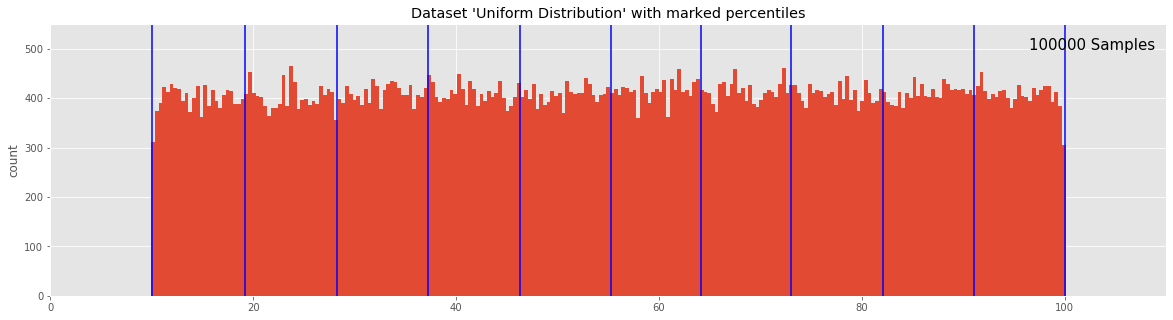
\includegraphics[width=\textwidth]{evaluation/images/Uniform_Distribution_distribution_percentiles.png}
   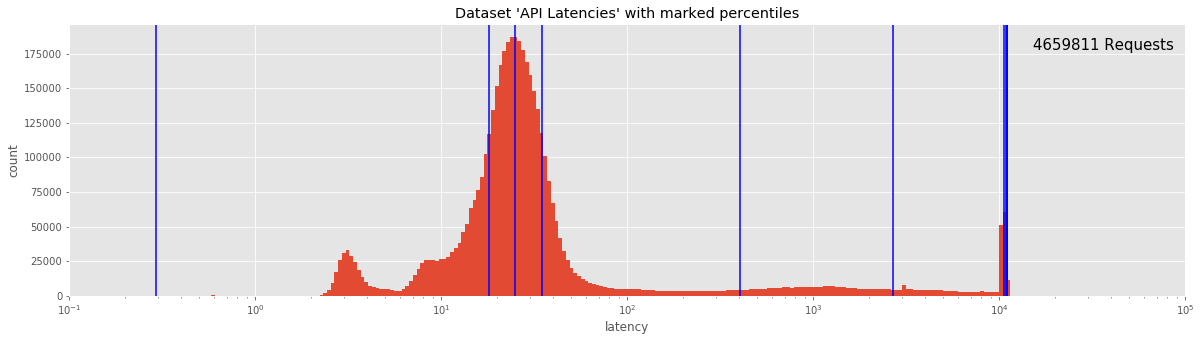
\includegraphics[width=\textwidth]{evaluation/images/API_Latencies_distribution_percentiles.png}
   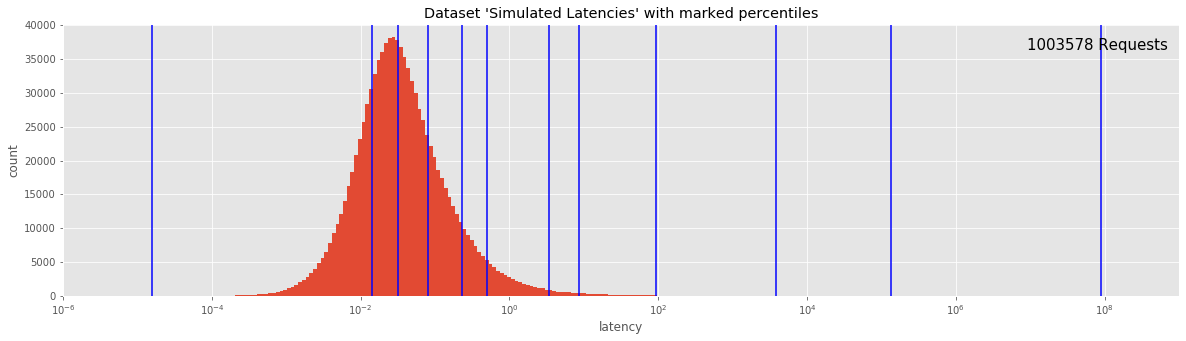
\includegraphics[width=\textwidth]{evaluation/images/Simulated_Latencies_distribution_percentiles.png}
   \caption{Datasets}
\end{figure}

\clearpage
\subsection{Size}

\begin{figure*}[t!]
  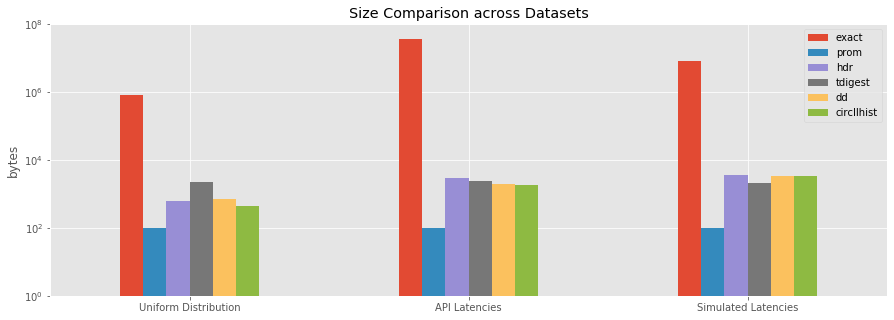
\includegraphics[width=\textwidth]{evaluation/images/all_size.png}
  \caption{Size Comparison}
\end{figure*}

\begin{figure}
  \centering
  \begin{tabular}{lrrrrrr}
\toprule
{} &     exact &  prom &  hdr &  tdigest &    dd &  circllhist \\
\midrule
Uniform Distribution &    800000 &    96 &  621 &     2224 &   716 &         453 \\
API Latencies        &  37278488 &    96 & 2994 &     2368 &  1902 &        1866 \\
Simulated Latencies  &   8028624 &    96 & 3699 &     2096 &  3428 &        3396 \\
\bottomrule
\end{tabular}

  \caption{Aggregation sizes in kb}
\end{figure}

\clearpage
\subsection{Performance}

\begin{figure}
  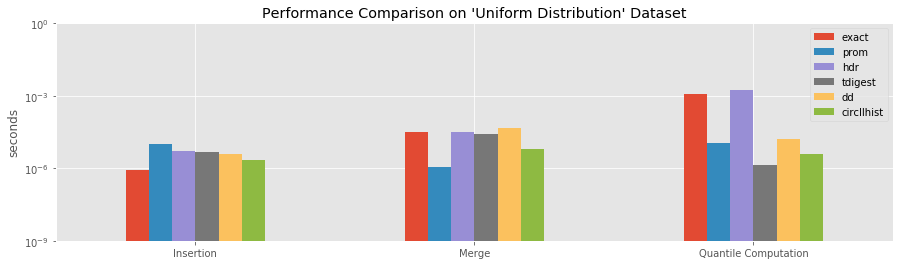
\includegraphics[width=\textwidth]{evaluation/images/Uniform_Distribution_perf.png}
  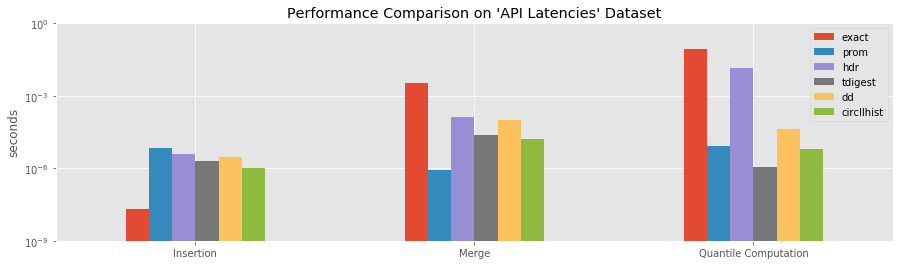
\includegraphics[width=\textwidth]{evaluation/images/API_Latencies_perf.png}
  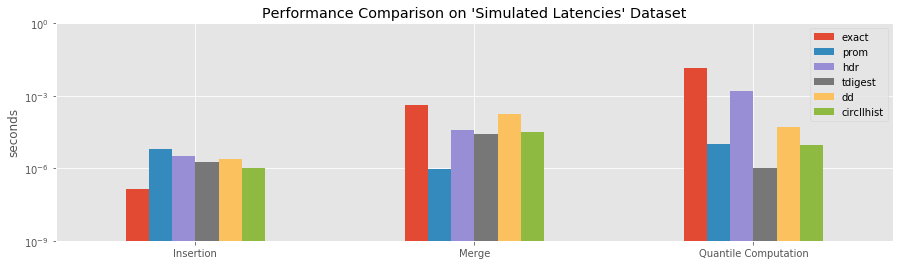
\includegraphics[width=\textwidth]{evaluation/images/Simulated_Latencies_perf.png}
  \caption{Performance Comparison}
\end{figure}

Tables in usec

Uniform\\
\begin{tabular}{lrrrrrr}
\toprule
{} &  exact &  prom &    hdr &  tdigest &   dd &  circllhist \\
\midrule
Insertion            &    0.9 &  10.5 &    7.7 &      4.6 &  3.8 &         2.2 \\
Merge                &   33.1 &   1.1 &  129.0 &     26.9 & 45.8 &         6.3 \\
Quantile Computation & 1180.3 &  11.3 & 9684.9 &      1.4 & 17.1 &         3.8 \\
\bottomrule
\end{tabular}


API Latencies\\
\begin{tabular}{lrrrrrr}
\toprule
{} &   exact &  prom &    hdr &  tdigest &    dd &  circllhist \\
\midrule
Insertion            &     0.0 &   6.9 &    3.7 &      2.0 &   3.0 &         1.0 \\
Merge                &  3487.6 &   0.9 &   34.1 &     24.0 & 104.6 &        16.1 \\
Quantile Computation & 83773.2 &   8.3 & 1931.4 &      1.1 &  42.6 &         6.1 \\
\bottomrule
\end{tabular}


Simulated API Latency Data\\
\begin{tabular}{lrrrrrr}
\toprule
{} &   exact &  prom &     hdr &  tdigest &    dd &  circllhist \\
\midrule
Insertion            &     0.1 &   6.5 &     3.5 &      1.9 &   2.5 &         1.0 \\
Merge                &   415.4 &   1.0 &   135.6 &     27.1 & 185.7 &        31.7 \\
Quantile Computation & 14222.5 &  10.0 & 11198.1 &      1.1 &  51.4 &         8.9 \\
\bottomrule
\end{tabular}


\clearpage
\subsection{Accuracy}

\begin{figure}
  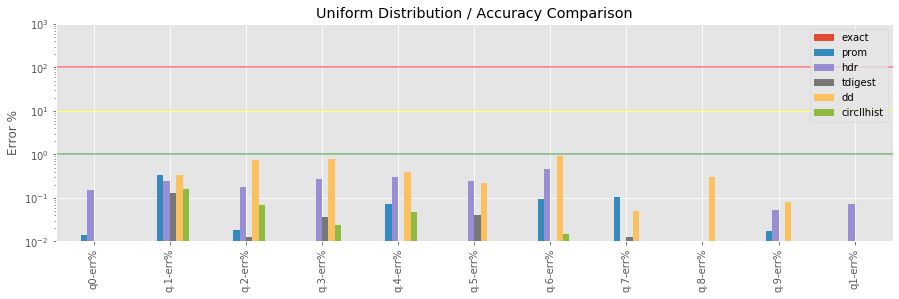
\includegraphics[width=\textwidth]{evaluation/images/Uniform_Distribution_accuracy.png}
  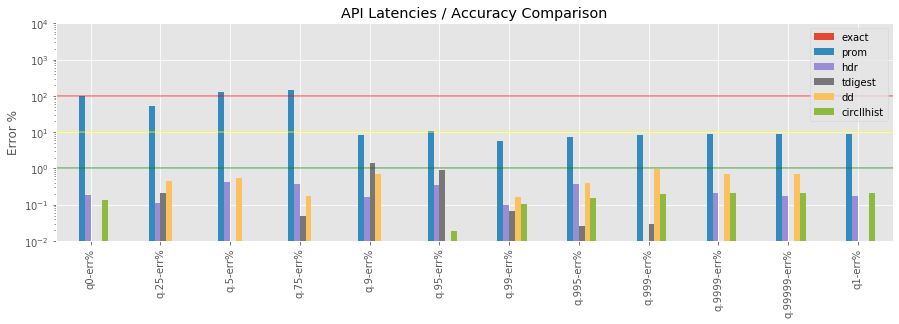
\includegraphics[width=\textwidth]{evaluation/images/API_Latencies_accuracy.png}
  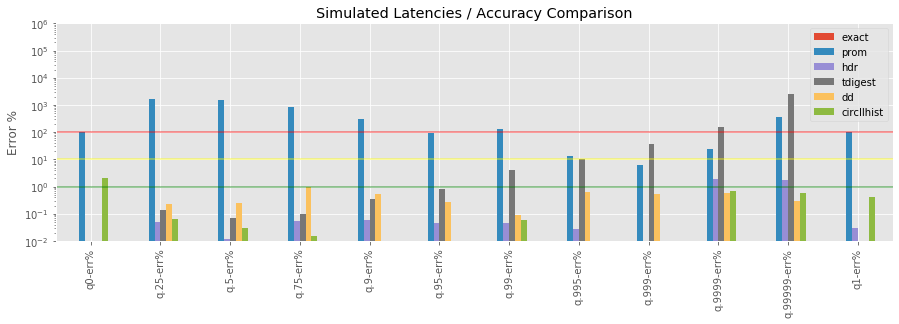
\includegraphics[width=\textwidth]{evaluation/images/Simulated_Latencies_accuracy.png}
  \caption{Accuracy Comparison}
\end{figure}

\begin{figure}
  Uniform\\
  \begin{tabular}{lrrrrr}
\toprule
{} &  prom &   hdr &  tdigest &    dd &  circllhist \\
\midrule
q0-err\%  & 0.014 & 0.156 &    0.000 & 0.000 &       0.005 \\
q.1-err\% & 0.339 & 0.248 &    0.129 & 0.342 &       0.160 \\
q.2-err\% & 0.018 & 0.178 &    0.013 & 0.736 &       0.069 \\
q.3-err\% & 0.006 & 0.273 &    0.036 & 0.794 &       0.024 \\
q.4-err\% & 0.074 & 0.297 &    0.003 & 0.394 &       0.048 \\
q.5-err\% & 0.000 & 0.243 &    0.040 & 0.216 &       0.007 \\
q.6-err\% & 0.094 & 0.468 &    0.006 & 0.931 &       0.015 \\
q.7-err\% & 0.105 & 0.006 &    0.013 & 0.050 &       0.000 \\
q.8-err\% & 0.004 & 0.010 &    0.001 & 0.307 &       0.009 \\
q.9-err\% & 0.017 & 0.053 &    0.006 & 0.081 &       0.000 \\
q1-err\%  & 0.000 & 0.073 &    0.000 & 0.000 &       0.001 \\
\bottomrule
\end{tabular}

  API Latencies\\
  \begin{tabular}{lrrrrr}
\toprule
{} &    prom &   hdr &  tdigest &    dd &  circllhist \\
\midrule
q0-err\%      & 100.000 & 0.038 &    0.000 & 0.000 &       0.134 \\
q.25-err\%    &  52.671 & 0.035 &    0.216 & 0.460 &       0.000 \\
q.5-err\%     & 126.469 & 0.038 &    0.000 & 0.538 &       0.003 \\
q.75-err\%    & 145.163 & 0.061 &    0.049 & 0.171 &       0.001 \\
q.9-err\%     &   8.230 & 0.007 &    1.382 & 0.685 &       0.006 \\
q.95-err\%    &  10.636 & 0.023 &    0.907 & 0.006 &       0.019 \\
q.99-err\%    &   5.662 & 0.031 &    0.066 & 0.164 &       0.105 \\
q.995-err\%   &   7.313 & 0.064 &    0.026 & 0.399 &       0.155 \\
q.999-err\%   &   8.584 & 0.010 &    0.030 & 0.979 &       0.202 \\
q.9999-err\%  &   8.862 & 0.019 &    0.007 & 0.715 &       0.216 \\
q.99999-err\% &   8.891 & 0.050 &    0.003 & 0.683 &       0.216 \\
q1-err\%      &   8.894 & 0.047 &    0.000 & 0.000 &       0.217 \\
\bottomrule
\end{tabular}

  Simulated API Latency Data\\
  \begin{tabular}{lrrrrr}
\toprule
{} &     prom &   hdr &  tdigest &    dd &  circllhist \\
\midrule
q0-err\%      &  100.000 & 0.407 &    0.000 & 0.000 &       2.110 \\
q.25-err\%    & 1706.372 & 0.232 &    0.141 & 0.238 &       0.062 \\
q.5-err\%     & 1523.356 & 0.012 &    0.069 & 0.243 &       0.029 \\
q.75-err\%    &  857.929 & 0.054 &    0.101 & 0.957 &       0.016 \\
q.9-err\%     &  296.620 & 0.689 &    0.342 & 0.546 &       0.009 \\
q.95-err\%    &   95.263 & 0.632 &    0.813 & 0.277 &       0.004 \\
q.99-err\%    &  133.561 & 0.146 &    4.152 & 0.087 &       0.059 \\
q.995-err\%   &   13.454 & 0.029 &   10.259 & 0.649 &       0.008 \\
q.999-err\%   &    6.136 & 0.406 &   36.221 & 0.519 &       0.002 \\
q.9999-err\%  &   23.154 & 1.933 &  149.000 & 0.599 &       0.670 \\
q.99999-err\% &  355.293 & 2.224 & 2559.294 & 0.301 &       0.570 \\
q1-err\%      &   98.875 & 0.347 &    0.000 & 0.000 &       0.409 \\
\bottomrule
\end{tabular}

\end{figure}

\section{Conclusion}

HDR Histograms, DDSketches and Circllhist are very similar approaches to the same problem of
summarizing distributions in a way that allows arbitrary aggregations and a wide range of
statistical operations like percentiles.

- All three methods are based on logarithmic histograms

- All three methods cover essentially unbounded data ranges

- All three methods offer fast insertion times

- All three methods offer a-priori bound on the relative error

In comparison to the other methods:

- circllhist is the oldest method, dating back to 2013 when it was first introduced in Circonus.

- circllhist allows exact less-than counts at decimal floating point numbers

- circllhist has the most performat C implementation available

Prometheus histograms

- require manual setting of thresholds and

- only offer good percentile accuracy if the percentiles happen to lie near those thresholds.

- non-sparse data structure makes using lot's of bins impractical

T-digest

- more complicated structure

- good results on well behaved datasets

- no a-priori error bounds on relative error after merge operations

- we have seen cases where the relative error grows to > 100x


\bibliographystyle{unsrt}
\begin{thebibliography}{1}

\bibitem{tdigest}
T. Dunning and O. Ertl.
\newblock  Computing extremeley accurate quantiles using t-digests.
\newblock \url{https://github.com/tdunning/t-digest}, 2017.

\bibitem{dd}
M. Charles, J.E. Rim, H.K. Lee.
\newblock DDSketch: A fast and fully-mergeable quantile sketch with relative-error guarantees.
\newblock Proceedings of the VLDB Endowment 12.12 (2019): 2195-2205.

\bibitem{hdr}
G. Tene,
\newblock HdrHistogram: A high dynamic range (hdr) histogram
\newblock \url{http://hdrhistogram.org/}, 2012

\bibitem{libcircllhist}
  Circonus.
  \newblock libcircllhist: An implementation of Circonus Log-Linear Histograms
  \newblock \url{https://github.com/circonus-labs/libcircllhist}, 2016

\bibitem{HF1996}
  Hyndman, R. J. and Fan, Y.
  \newbloack Sample quantiles in statistical packages
  \newblock American Statistician 50, 361–365. 10.2307/2684934, 1996

\end{thebibliography}
\end{document}
